\section{Experiments}
\label{sec:exp}

\paragraph{Data.}
All matrices are public and version-pinned (Appendix~\ref{app:repro}). \textbf{MTEB} \citep{muennighoff2022mteb,mtebresults}: one score per (embedding model, task), the task's main metric on its test split (averaged over language subsets; a task enters only with the modal subset signature). From 531 models $\times$ 1,172 tasks (11\% filled) we keep tasks with $\ge100$ models and models with $\ge60$ of those tasks: \textbf{MTEB-main} (189 models $\times$ 280 tasks, 77\% filled, on average 215 observed tasks per model); \textbf{MTEB-dense} ($\ge150$ models/task, $\ge80$ tasks/model: 175 $\times$ 164, 90\%) and \textbf{MTEB-eng} (English tasks only: 185 $\times$ 91). LLM leaderboards are small in $N$: \textbf{OpenLLM-LB} (6 benchmarks $\times$ 4,496 models, complete; \citealp{openllm2024}), \textbf{HELM-Lite-22} (22 scenario/sub-scenario scores $\times$ 91 models; \citealp{helmlite,liang2022helm}), its 10-scenario version, and \textbf{LiveBench-7} (7 task scores $\times$ 158 models with $\ge5$ of them; \citealp{white2024livebench}). In every matrix (Table~\ref{tab:data}) one factor carries 57--74\% of the correlation spectrum, but 90\% of it needs $n_{90}=3$--20 components: a dominant general factor plus a long tail.

\begin{table}[t]
\centering\small
\caption{Matrices. $\lambda_1/N$: top eigenvalue share of the pairwise correlation matrix; PR: participation ratio; $n_{90}$: components for 90\% of the spectrum; $\rho$: off-diagonal correlation.}
\label{tab:data}
\begin{tabular}{lrrrrrrr}\toprule
Dataset & Models & Bench. & Density & $\lambda_1/N$ & PR & $n_{90}$ & mean $\rho$ \\\midrule
MTEB-main & 189 & 280 & 0.77 & 0.57 & 2.9 & 20 & 0.56 \\
MTEB-dense & 175 & 164 & 0.90 & 0.60 & 2.6 & 15 & 0.58 \\
MTEB-eng & 185 & 91 & 0.70 & 0.68 & 2.1 & 10 & 0.65 \\
HELM-Lite-22 & 91 & 22 & 1.00 & 0.58 & 2.8 & 8 & 0.52 \\
HELM-Lite-10 & 91 & 10 & 1.00 & 0.63 & 2.3 & 4 & 0.55 \\
LiveBench-7 & 158 & 7 & 0.89 & 0.73 & 1.8 & 4 & 0.68 \\
OpenLLM-LB & 4496 & 6 & 1.00 & 0.74 & 1.8 & 3 & 0.67 \\
\bottomrule\end{tabular}

\end{table}

\paragraph{Protocol.}
\emph{Rows are held out}, never cells: models are split into 5 folds (3 repeats with different fold seeds for MTEB, 10 for HELM/LiveBench, 1 for OpenLLM), all fitting, tuning and selection use training rows only, and each held-out model is a ``new model'' that reveals $k$ scores. For every held-out model with observed set $C$ we draw a set $T_0$ of \emph{held-out targets} (30\% of $C$; two draws per model; for $N\le12$ every single benchmark in turn) and let each selector choose $S$ from the pool $C\setminus T_0$. \emph{All selectors and predictors are scored on the same $T_0$.} Selection is thus restricted to what the model actually has scores for, and neither $S$ nor the baseline determines the targets (\S\ref{sec:exp_pitfall} shows why this matters). Curves compare the same (model, $T_0$) cells at every $k$. We report the standardized MSE and $R^2=1-\mathrm{MSE}/\mathrm{MSE}_{\textsc{mean}}$, where \textsc{mean} predicts each target by its training mean; random selection averages 10 draws per cell. Uncertainty: 95\% percentile bootstrap over held-out \emph{models}, resampled jointly for paired differences (Wilcoxon $p$-values are in the released tables). Besides random splits we use \emph{new-organisation} splits (5 folds by organisation prefix, MTEB) and a \emph{temporal} split (training on the oldest 70\% of models by release/submission date, testing on the rest: 53 MTEB models, 1,332 OpenLLM models).

\subsection{How accurate is inference from $k$ benchmarks, and does selection matter?}
\label{sec:exp_main}
Figure~\ref{fig:main} and Table~\ref{tab:main} give the central result. On MTEB-main the average held-out model has 215 observed tasks, 30\% of which (about 65) are the held-out targets, and the mean baseline has RMSE 17.4 score points per target. With \emph{one} well-chosen task, $R^2=0.52$ (RMSE 11.0 points); with five, 0.71 (8.0 points); with ten, 0.76 (7.2 points). After that returns diminish quickly: at $k=40$ both greedy and random reach $R^2\approx0.80$ (6.7 vs.\ 6.4 points). The plateau is reached by every selector and by the best predictors (Appendix Table~\ref{tab:pred}): the unexplained 20\% is consistent with benchmark-specific variation that the other benchmarks do not carry (we cannot separate it from evaluation noise). It is far smaller for \emph{aggregates}: the mean of the held-out scores is predicted with mean absolute error 1.7 points at $k=5$ and 1.3 at $k=10$ (random: 2.7 and 1.8; mean baseline: 10.5), because benchmark-specific errors average out (Appendix~\ref{app:more}).

\begin{figure}[t]
\centering
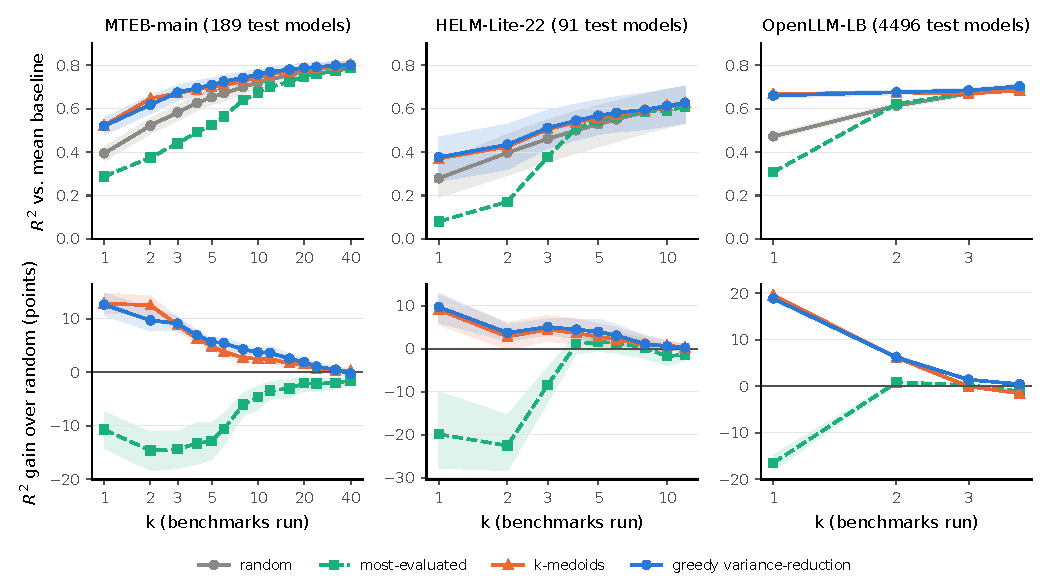
\includegraphics[width=\linewidth]{figs/main_curves.pdf}
\caption{Held-out accuracy vs.\ number of benchmarks run $k$ (Gaussian predictor). Top: $R^2$ vs.\ the mean baseline; bottom: paired $R^2$ gain over random selection; bands: 95\% bootstrap CIs over models. On complete matrices (OpenLLM-LB, HELM) ``most-evaluated'' is column order. Other matrices: Fig.~\ref{fig:app_curves}.}
\label{fig:main}
\end{figure}

\begin{table}[t]
\centering\small
\caption{$R^2$ [95\% CI] at $k$ benchmarks run, Gaussian predictor, random splits of models. Bold: best selector per column (ties at two decimals); ``--'': $k$ not available for this matrix.}
\label{tab:main}
\resizebox{\linewidth}{!}{\begin{tabular}{llcccc}\toprule
Dataset (split) & Selector & $k{=}1$ & $k{=}3$ & $k{=}5$ & $k{=}10$ \\\midrule
MTEB-main (rand) & random & 0.39 \scriptsize[0.36,0.42] & 0.58 \scriptsize[0.54,0.62] & 0.65 \scriptsize[0.62,0.68] & 0.72 \scriptsize[0.69,0.75] \\
 & most-evaluated & 0.29 \scriptsize[0.24,0.33] & 0.44 \scriptsize[0.38,0.48] & 0.52 \scriptsize[0.47,0.57] & 0.67 \scriptsize[0.63,0.71] \\
 & k-medoids & \textbf{0.52} \scriptsize[0.48,0.56] & \textbf{0.67} \scriptsize[0.64,0.71] & 0.70 \scriptsize[0.67,0.73] & 0.75 \scriptsize[0.72,0.77] \\
 & greedy variance-reduction & \textbf{0.52} \scriptsize[0.48,0.56] & \textbf{0.67} \scriptsize[0.64,0.71] & \textbf{0.71} \scriptsize[0.68,0.74] & \textbf{0.76} \scriptsize[0.73,0.78] \\
\midrule
HELM-Lite-22 (rand) & random & 0.28 \scriptsize[0.19,0.35] & 0.46 \scriptsize[0.35,0.55] & 0.53 \scriptsize[0.42,0.62] & \textbf{0.61} \scriptsize[0.51,0.69] \\
 & most-evaluated & 0.08 \scriptsize[0.04,0.12] & 0.38 \scriptsize[0.26,0.46] & 0.54 \scriptsize[0.44,0.63] & 0.59 \scriptsize[0.49,0.68] \\
 & k-medoids & 0.37 \scriptsize[0.26,0.46] & \textbf{0.51} \scriptsize[0.42,0.58] & 0.56 \scriptsize[0.47,0.63] & \textbf{0.61} \scriptsize[0.52,0.69] \\
 & greedy variance-reduction & \textbf{0.38} \scriptsize[0.26,0.47] & \textbf{0.51} \scriptsize[0.42,0.59] & \textbf{0.57} \scriptsize[0.48,0.64] & \textbf{0.61} \scriptsize[0.52,0.69] \\
\midrule
OpenLLM-LB (rand) & random & 0.47 \scriptsize[0.46,0.49] & 0.67 \scriptsize[0.66,0.68] & -- & -- \\
 & most-evaluated & 0.31 \scriptsize[0.29,0.33] & 0.67 \scriptsize[0.66,0.68] & -- & -- \\
 & k-medoids & \textbf{0.67} \scriptsize[0.66,0.68] & 0.67 \scriptsize[0.66,0.68] & -- & -- \\
 & greedy variance-reduction & 0.66 \scriptsize[0.65,0.67] & \textbf{0.68} \scriptsize[0.67,0.69] & -- & -- \\
\midrule
LiveBench-7 (rand) & random & 0.47 \scriptsize[0.40,0.53] & 0.61 \scriptsize[0.54,0.67] & -- & -- \\
 & most-evaluated & 0.50 \scriptsize[0.41,0.58] & \textbf{0.64} \scriptsize[0.58,0.69] & -- & -- \\
 & k-medoids & \textbf{0.53} \scriptsize[0.46,0.60] & 0.60 \scriptsize[0.54,0.66] & -- & -- \\
 & greedy variance-reduction & \textbf{0.53} \scriptsize[0.45,0.59] & 0.59 \scriptsize[0.53,0.65] & -- & -- \\
\bottomrule
\end{tabular}
}
\end{table}

\emph{Selection matters most at the smallest budgets.} On MTEB-main, greedy selection lowers the MSE of random selection by 21\% [17, 25] at $k=1$, 16\% [14, 19] at $k=5$, 13\% [12, 15] at $k=10$, 8\% [6, 11] at $k=20$, and not detectably at $k=40$ ($-1\%$ [$-4$, 1]); the number of tasks needed for $R^2\ge0.75$ falls from 16 to 10 (Table~\ref{tab:kneeded}). $k$-medoids on $1-|\rho|$ is nearly as good (equal or better at $k\le3$, 3--5\% worse for $k\in\{5,10\}$); the max-variance (``entropy'') rule of \citet{krause2008near} is much worse at small $k$ (it picks idiosyncratic tasks) and their mutual-information rule is slightly worse than ours; choosing the benchmarks with the largest average correlation is as good as greedy at $k=1$ but \emph{worse than random} from $k=6$ on ($-9.9\%$ [$-13.8$, $-6.3$] at $k=10$), because it picks redundant, mutually correlated benchmarks. Most strikingly, running \emph{the most commonly reported tasks} is worse than random at every $k$ we tried: $-18\%$ [$-24$, $-12$] at $k=1$ and $-37\%$ [$-48$, $-27$] at $k=5$ (MTEB-main, where popularity is informative). Across matrices (Table~\ref{tab:main}, Fig.~\ref{fig:app_curves}) the MSE reduction at $k=1$ is 12--36\% and shrinks with $k$. In the three tiny LLM matrices the useful range of $k$ is short: OpenLLM-LB: one well-chosen benchmark gives $R^2=0.66$ vs.\ 0.47 (random), three give 0.68 vs.\ 0.67, and the plateau is 0.70; HELM-Lite-22 greedy gain is 13\% [8, 19] at $k=1$ and not significant at $k=10$ (1\% [$-1$, 4]); on LiveBench-7 selection is not helpful beyond $k=1$ and greedy is \emph{worse} than random at $k=3$ ($-4\%$ [$-7$, $-2$]).

\begin{table}[t]
\centering\small
\caption{Smallest $k$ reaching a target $R^2$ (``$>K$'': not reached up to the largest $k$ evaluated).}
\label{tab:kneeded}
\begin{tabular}{llccc}\toprule
Dataset (protocol) & Selector & $R^2\ge0.6$ & $R^2\ge0.7$ & $R^2\ge0.75$ \\\midrule
HELM-Lite-22 (rand) & random & 10 & $>$12 & $>$12 \\
 & greedy variance-reduction & 10 & $>$12 & $>$12 \\
MTEB-dense (rand) & random & 4 & 10 & 20 \\
 & greedy variance-reduction & 2 & 6 & 16 \\
MTEB-eng (rand) & random & 2 & 5 & 10 \\
 & greedy variance-reduction & 1 & 3 & 5 \\
MTEB-main (org) & random & 6 & 20 & $>$40 \\
 & greedy variance-reduction & 3 & 10 & $>$40 \\
MTEB-main (rand) & random & 4 & 10 & 16 \\
 & greedy variance-reduction & 2 & 5 & 10 \\
MTEB-main (time) & random & 12 & $>$40 & $>$40 \\
 & greedy variance-reduction & 6 & $>$40 & $>$40 \\
OpenLLM-LB (rand) & random & 2 & $>$4 & $>$4 \\
 & greedy variance-reduction & 1 & 4 & $>$4 \\
OpenLLM-LB (time) & random & 2 & $>$4 & $>$4 \\
 & greedy variance-reduction & 1 & 4 & $>$4 \\
\bottomrule
\end{tabular}

\end{table}

\subsection{Which predictor?}
\label{sec:exp_pred}
Appendix Table~\ref{tab:pred} fixes the selection (random or greedy) and varies the predictor (hyper-parameters tuned on the training rows). The naive ``average of what was run'' (\textsc{AvgShift}) saturates at $R^2\approx0.6$: no amount of averaging substitutes for modelling which benchmarks resemble which. The covariance-based predictors are close to each other, and no predictor is uniformly best (paired CIs in Appendix Table~\ref{tab:ci_pred}). \textsc{Hybrid} is slightly but significantly better than \textsc{Gauss} for $k\ge10$ (+0.004 to +0.023 $R^2$, largest at $k=40$), \textsc{FA} and \textsc{ISVD} are 0.01--0.04 behind it for $k\ge10$ (the tuned factor rank is 3--12, so the covariance is \emph{not} well described by one or two factors), and \textsc{kNN} is \emph{better} at $k=1$ (+0.05 [0.03, 0.07] under random and +0.08 [0.05, 0.10] under greedy selection) and about equal for $k=5$--$20$; a single benchmark apparently has a non-linear relation to the others that a linear-Gaussian conditional misses. Greedy selection, which assumes the Gaussian model, improves every covariance-based predictor and \textsc{kNN} too.


\subsection{Does it survive distribution shift?}
\label{sec:exp_shift}
Table~\ref{tab:shift} repeats the MTEB-main experiment with \emph{new-organisation} and \emph{later-release} test models. The mean baseline degrades (its standardized MSE is 1.36 for new organisations and 3.25 for later releases vs.\ 1.18: later models differ systematically from the history, presumably by scoring higher), and $R^2$ at $k=40$ drops to $\approx0.72$ and $\approx0.65$. The benefit of selection survives at small budgets (new organisation: 21\%, 17\%, 22\%, 18\% MSE reduction at $k=1,2,3,5$, all CIs exclude 0), vanishes at $k=20$ for new organisations (1\% [$-3$, 5]), and persists for later releases (13\% [8, 17] at $k=20$). Selection from the history alone remains valuable at $k\le5$ even when the new model comes from an unseen lab; but the budget needed for a given $R^2$ increases ($R^2\ge0.7$ needs 10 tasks for new organisations, and $>40$ for later releases, Table~\ref{tab:kneeded}).

\begin{table}[t]
\centering\small
\caption{MTEB-main under three protocols ($R^2$, Gaussian predictor).}
\label{tab:shift}
\begin{tabular}{llccccc}\toprule
Protocol & Selector & $k{=}1$ & $k{=}3$ & $k{=}5$ & $k{=}10$ & $k{=}20$ \\\midrule
random models & random & 0.39 & 0.58 & 0.65 & 0.72 & 0.77 \\
 & most-evaluated & 0.29 & 0.44 & 0.52 & 0.67 & 0.75 \\
 & k-medoids & 0.52 & 0.67 & 0.70 & 0.75 & 0.78 \\
 & greedy variance-reduction & 0.52 & 0.67 & 0.71 & 0.76 & 0.79 \\
\midrule
new organisation & random & 0.35 & 0.54 & 0.60 & 0.66 & 0.71 \\
 & most-evaluated & 0.28 & 0.32 & 0.45 & 0.61 & 0.65 \\
 & k-medoids & 0.50 & 0.62 & 0.66 & 0.68 & 0.71 \\
 & greedy variance-reduction & 0.49 & 0.64 & 0.67 & 0.70 & 0.71 \\
\midrule
later release & random & 0.31 & 0.51 & 0.55 & 0.59 & 0.64 \\
 & most-evaluated & 0.25 & 0.11 & 0.39 & 0.54 & 0.61 \\
 & k-medoids & 0.47 & 0.55 & 0.60 & 0.64 & 0.66 \\
 & greedy variance-reduction & 0.46 & 0.52 & 0.60 & 0.65 & 0.68 \\
\bottomrule
\end{tabular}

\end{table}

\subsection{Under which data conditions do the conclusions hold?}
\label{sec:exp_cond}
Figure~\ref{fig:cond} varies one data property of MTEB-main at a time. (i)~\emph{History size}: the greedy gain over random is 8--14\% for every history size (10\% [6, 18] with 25 training models, 14\% [11, 17] with all $\sim$151; CIs of $\le100$ models include small values), but absolute accuracy changes a lot: greedy $R^2$ at $k=10$ is 0.49, 0.67, 0.71, 0.77 for 25, 50, 100, all training models. (ii)~\emph{Missingness}: dropping 30\% of the history's observed cells leaves the gain at 10\%, dropping 60\% cuts it to 4\% [0, 7] and $R^2$ from 0.74 to 0.61 (greedy at $k=10$). (iii)~\emph{Pool composition}: greedy helps in every pool except when benchmarks are drawn only from the 59 classification tasks (gain 2\% [$-5$, 8]); the gain is largest for the non-English pool (12\% [6, 17]) and the clustering+STS+pair pool (10\% [6, 14]). (iv)~A \emph{logit transform} of the scores does not help ($R^2=0.75$ vs.\ 0.74 at $k=10$, CIs overlap; both evaluated in score points). (v)~\emph{Target construction}: holding out 10\% or 50\% of each model's observed benchmarks, or whole name-based task families (so that no near-duplicate of a target is in the pool), leaves the $k=10$ gain at 10\% [6, 14], 14\% [10, 18] and 14\% [10, 18]. (vi)~Estimating the selection covariance from the training rows costs little: using a covariance estimated with the test models included (``oracle'') improves the MSE at $k\le10$ by only 1--4\% over our greedy rule, whereas selecting with the low-rank factor-model covariance is 5--9\% \emph{worse} at $k=10,20$ on MTEB-main (Appendix Table~\ref{tab:oracle}).

\begin{figure}[t]
\centering
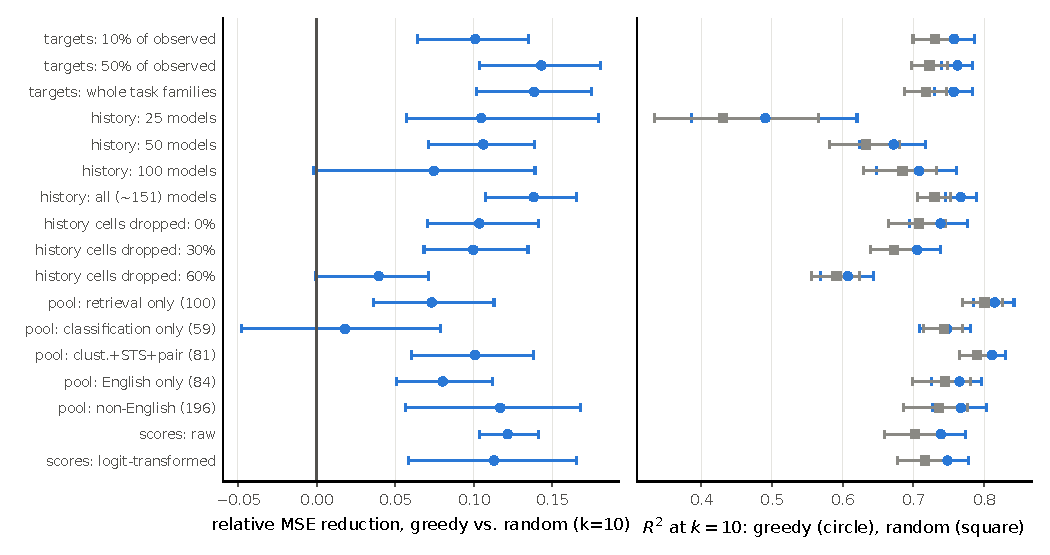
\includegraphics[width=\linewidth]{figs/conditions.pdf}
\caption{Data conditions (MTEB-main, $k=10$). Left: relative MSE reduction of greedy vs.\ random with 95\% CI. Right: $R^2$ of greedy (circle) and random (square).}
\label{fig:cond}
\end{figure}

\subsection{Theory against experiment}
\label{sec:exp_theory}
\begin{figure}[t]
\centering
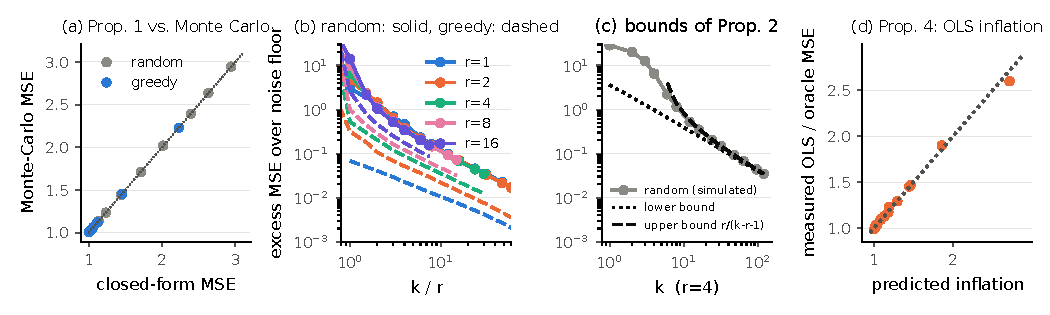
\includegraphics[width=\linewidth]{figs/synthetic_theory.pdf}
\caption{Synthetic checks. (a)~Prop.~\ref{prop:closed} vs.\ Monte Carlo. (b)~Excess error over the noise floor vs.\ $k/r$ ($N{=}400$, $g_i=10$): random-$S$ curves for different ranks collapse. (c)~Random-$S$ excess ($r=4$) between the bounds of Prop.~\ref{prop:random}. (d)~OLS/oracle MSE ratio vs.\ $1+k/(M-k-1)$ (Prop.~\ref{prop:ols}).}
\label{fig:synth}
\end{figure}
\emph{Synthetic factor models} (Fig.~\ref{fig:synth}). The closed form of Prop.~\ref{prop:closed} matches Monte Carlo to within 0.006 in MSE for all random and greedy sets tested. The sandwich of Prop.~\ref{prop:random} holds in all 94 (rank, strength, $k$) cells with $k\ge r+2$ (within 3 MC standard errors), and the smallest $k$ with simulated excess $\le\epsilon\sigma^2$ lies in $[r/\epsilon-1/g,\ r(1+1/\epsilon)+1]$ in 21 of 24 settings and exceeds the upper end by one (MC noise at the bound) in the other three: e.g.\ $r=8,\ \epsilon=0.1$ requires $k=90$, i.e.\ $\approx 11r$. Greedy selection reaches the same excess with 0.08--0.48 (median 0.29) times as many benchmarks (e.g.\ 38 instead of 90 for $r=8,\epsilon=0.1$), a far larger gain than on real matrices, whose spectra have one dominant factor that random sets already capture. The OLS inflation $1+k/(M-k-1)$ of Prop.~\ref{prop:ols} agrees with simulation to a mean absolute deviation of 0.016 (max.\ 4.3\% relative). The spectral bound of Prop.~\ref{prop:tail} is never violated by the exhaustive optimum (0 of 480 instances) and is on average 82\% of it. Greedy selection recovers 99.7\% of the variance reduction of the exhaustive optimum on average (min.\ 0.91, 480 small instances; random: 0.87; the Das--Kempe bound is $0.18$ on average, hence loose), and a swap local search from the greedy set improves the residual objective by 1.4\% on average (max.\ 13\%) at $N=60$. The gain of greedy over random depends on the structure as the theory suggests (Appendix Table~\ref{tab:e5}): at $k=8$ the reduction of the residual objective is 3--8\% for one factor, 4--16\% for two, 5--29\% for four and 10--57\% for eight; it grows with factor strength $g$ and rank $r$ and shrinks when leverage is heterogeneous (log-sd $\kappa$ of the loading scales).

\emph{Real matrices.} The error that the fitted Gaussian predicts for itself, $\mathrm{tr}(\Sigma_{T|S})/|T|$, tracks the held-out MSE closely for both selectors (Appendix Fig.~\ref{fig:calib}): its ratio to the held-out error averages 0.97 (MTEB-main), 0.89 (MTEB-dense), 1.10 (MTEB-eng), 1.07 (HELM-22), and 1.03 (OpenLLM), within 0.62--1.26 over all $k$ and matrices. The model-implied curve can therefore be used to \emph{plan} $k$ for a target accuracy before running anything. Prop.~\ref{prop:tail} bounds in-sample residuals of any selection from below (Appendix Fig.~\ref{fig:spectral}); the in-sample greedy residual is 1.2--1.6$\times$ the bound on MTEB-main for $k\le40$, while random selection is 1.5--2.0$\times$.


\subsection{A protocol pitfall: scoring the complement}
\label{sec:exp_pitfall}
A natural protocol lets each selector pick $S$ from \emph{all} observed benchmarks and scores the model on the \emph{remaining} $C\setminus S$. Then selectors are scored on different targets, and a rule that removes the hardest-to-explain benchmarks into $S$ leaves the easy ones as targets. Appendix Table~\ref{tab:bias} compares both protocols for the same selected sets. With complement targets greedy appears to beat random at $k=40$ on MTEB-main by a MSE of 0.18 vs.\ 0.23 and at $k=12$ on HELM-Lite-22 by 0.27 vs.\ 0.42; on fixed targets the advantage is nil (0.24 vs.\ 0.24 and 0.41 vs.\ 0.42). The inflation is largest exactly where the budget is large relative to $N$.

